\documentclass{article}
\usepackage{cmap}
\usepackage[utf8]{inputenc}
\usepackage[english,ukrainian]{babel}
\usepackage{graphicx}
\usepackage{geometry}
\usepackage{listings}
\usepackage{float}
\usepackage{amsmath}
\geometry{
	a4paper,
	left=20mm,
	right=20mm,
	top=15mm,
	bottom=15mm,
}
\lstset{
	language=c,
	tabsize=4,
	keepspaces,
	showstringspaces=false,
}
\graphicspath{ {./pictures} }
\setlength{\parindent}{4em}

\newcommand\subject{Організація комп’ютерних мереж}
\newcommand\lecturer{асистент кафедри ПЗ \\ Задорожний І.М.}
\newcommand\teacher{асистент кафедри ПЗ \\ Задорожний І.М.}
\newcommand\mygroup{ПЗ-22}
\newcommand\lab{7}
\newcommand\theme{Дослідження роботи FTP-сервера та протоколу RDP}
\newcommand\purpose{Ознайомитися з основами протоколу FTP, дослідити формат
	повідомлень FTP та принцип роботи утиліти FTP}

\begin{document}
\begin{normalsize}
	\begin{titlepage}
		\thispagestyle{empty}
		\begin{center}
			\textbf{МІНІСТЕРСТВО ОСВІТИ І НАУКИ УКРАЇНИ\\
				НАЦІОНАЛЬНИЙ УНІВЕРСИТЕТ "ЛЬВІВСЬКА ПОЛІТЕХНІКА"}
		\end{center}
		\begin{flushright}
			\textbf{ІКНІ}\\
			Кафедра \textbf{ПЗ}
		\end{flushright}
		\vspace{200pt}
		\begin{center}
			\textbf{ЗВІТ}\\
			\vspace{10pt}
			до лабораторної роботи № \lab\\
			\textbf{на тему}: “\textit{\theme}”\\
			\textbf{з дисципліни}: “\subject”
		\end{center}
		\vspace{112pt}
		\begin{flushright}
			
			\textbf{Лектор}:\\
			\lecturer\\
			\vspace{28pt}
			\textbf{Виконав}:\\
			
			студент групи \mygroup\\
			Коваленко Д.М.\\
			\vspace{28pt}
			\textbf{Прийняв}:\\
			
			\teacher\\
			
			\vspace{28pt}
			«\rule{1cm}{0.15mm}» \rule{1.5cm}{0.15mm} 2023 р.\\
			$\sum$ = \rule{1cm}{0.15mm}……………\\
			
		\end{flushright}
		\vspace{\fill}
		\begin{center}
			\textbf{Львів — 2023}
		\end{center}
	\end{titlepage}
		
	\begin{description}
		\item[Тема.] \theme.
		\item[Мета.] \purpose.
	\end{description}

\section*{Теоретичні відомості}
\begin{itemize}
	\item Поясніть призначення протоколу FTP.
	
	FTP розшифровується як File Transfer Protocol — протокол  прикладного рівня для передач файлів у мережах TCP. FTP є клієнт-серверним протоколом. Клієнт “просить” у сервера файли, сервер їх надає. З його допомогою можна підключатися до інших комп’ютерів, щоб скачувати та завантажувати файли, а також керувати ними: встановлювати права доступу, створювати та редагувати текстові документи, додавати нові папки.
	
	Активний режим FTP влаштований так, що спочатку клієнт звертається до сервера, щоб встановити з’єднання, а потім вже сервер звертається до клієнта, щоб встановити інформаційне з’єднання. У такому режимі роботи FTP, якщо на комп’ютері користувача стоїть файрвол, він може заблокувати спробу сервера підключитися до нетиповому порту. Без фаервола все працюватиме без проблем.
	
	Пасивний режим FTP відрізняється від активного тим, що обидва з’єднання ініціює клієнт. Це вирішує проблему з файрволом, оскільки з’єднання, які встановлює клієнт, не блокуються.
	
	\item В чому полягає різниця між протоколами SFTP та FTPS?
	
	SFTP (Secure File Transfer Protocol) та FTPS (File Transfer Protocol Secure) є двома різними протоколами передачі файлів через мережу, які використовують шифрування для захисту даних під час передачі. Однак, вони відрізняються за способом реалізації та рівнем безпеки.
	
	SFTP - це протокол, який передає файли через SSH-канал. Він використовує шифрування на рівні пакетів, що забезпечує високий рівень безпеки. SFTP працює на порті 22, що є стандартним портом для SSH-з'єднань. SFTP є більш безпечним в порівнянні з FTPS, оскільки він не використовує повідомлення у відкритому вигляді для керування з'єднанням.
	
	FTPS - це протокол, який передає файли через TLS-або SSL-канал, що забезпечує захист даних від перехоплення. FTPS може працювати в двох режимах: як явний FTPS, де клієнт з'єднується з сервером на порту 21 і здійснює перехід до захищеного каналу з'єднання; та як неявний FTPS, де клієнт з'єднується з сервером на порті 990 і вже на цьому порті відбувається захищений обмін даними. FTPS може бути менш безпечним, оскільки він використовує повідомлення у відкритому вигляді для керування з'єднанням, що може бути вразливим до перехоплення.
	\item Скільки з’єднань використовує протокол FTP. Поясніть їх
	призначення?
	\begin{itemize}
		\item Керуючe з'єднання (Control Connection): Це з'єднання встановлюється між клієнтом та сервером для передачі команд, які використовуються для керування сеансом передачі файлів. Керуючий з'єднання зазвичай встановлюється на порту 21. Завдання керуючого з'єднання включає передачу команд від клієнта до сервера (наприклад, запит на список файлів або завантаження файлу), а також передачу відповідей від сервера клієнту (наприклад, список файлів або результати завантаження файлу).
		\item З'єднання передачі даних (Data Connection): Після встановлення керуючого з'єднання, клієнт та сервер можуть встановити одне або декілька з'єднань передачі даних для фактичної передачі файлів. Ці з'єднання можуть бути засновані на різних протоколах (наприклад, TCP або UDP), і вони можуть використовувати різні порти в залежності від конфігурації сервера та клієнта. Наприклад, при використанні активного режиму передачі даних, клієнт відкриває з'єднання на порту, вказаному сервером, а сервер відкриває з'єднання на порту, вказаний клієнтом для передачі даних.
	\end{itemize}
\end{itemize}


\section*{Хід виконання}
\begin{figure}[H]
	\centering
	
\includegraphics[width=\textwidth]{1}
	\caption{Створення серверу за допомогою FileZilla}
\end{figure}
\begin{figure}[H]
	\centering
	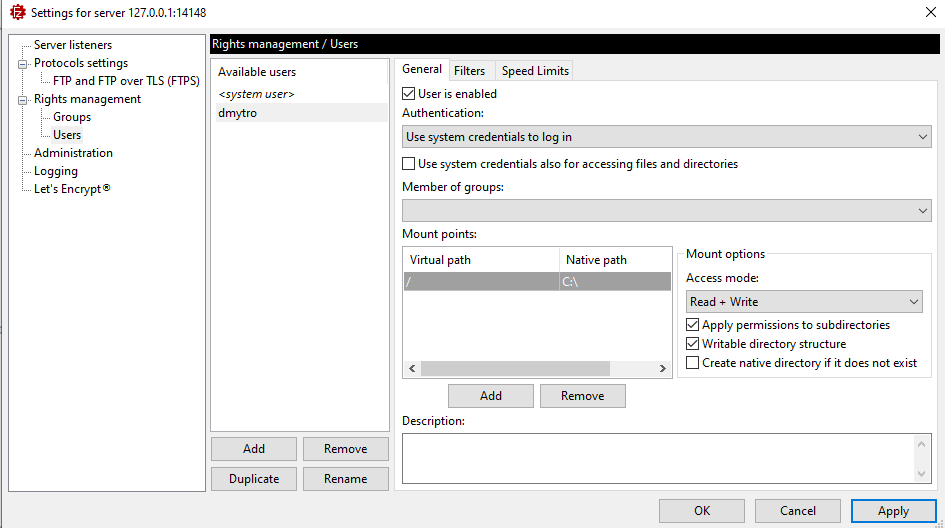
\includegraphics[width=\textwidth]{2}
	\caption{Користувач та кореневий каталог для нього}
\end{figure}
\begin{figure}[H]
	\centering
	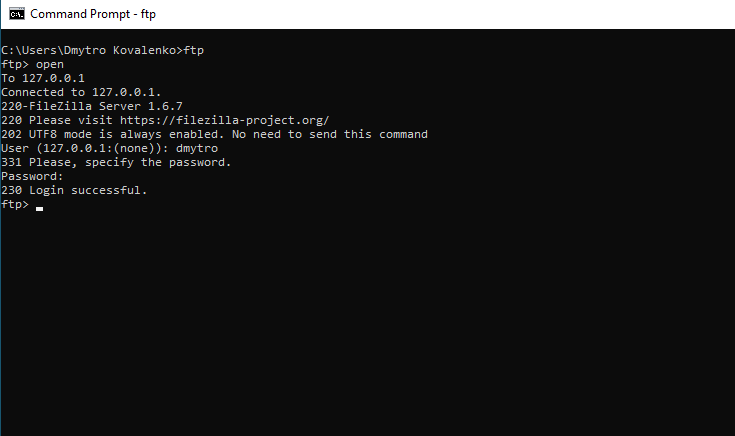
\includegraphics[width=\textwidth]{3}
	\caption{Під'єднання до ftp серверу}
\end{figure}
\begin{figure}[H]
	\centering
	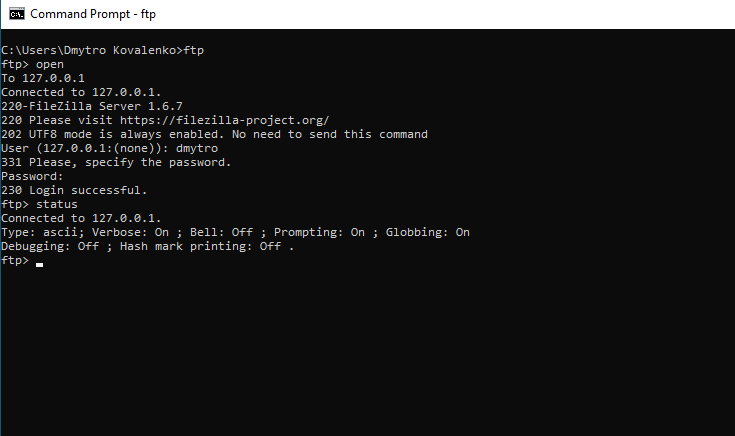
\includegraphics[width=\textwidth]{4}
	\caption{Перегляд параметрів з'єднання}
\end{figure}
\begin{figure}[H]
	\centering
	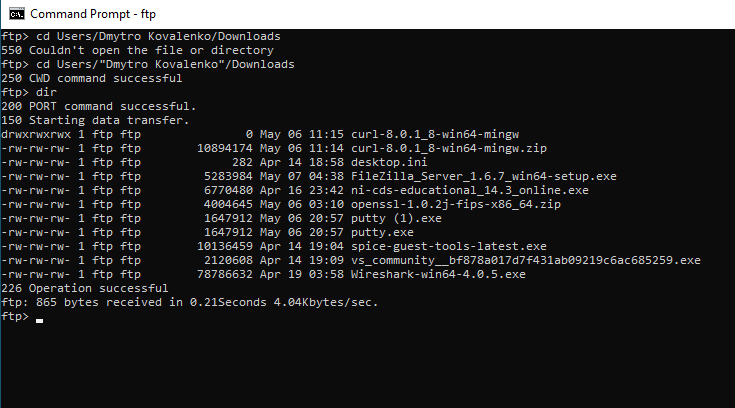
\includegraphics[width=\textwidth]{5}
	\caption{Зміна робочого каталогу та перегляд списку файлів}
\end{figure}
\begin{figure}[H]
	\centering
	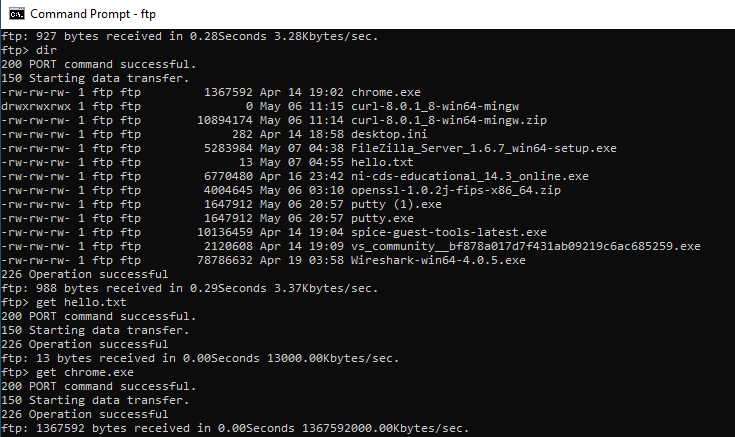
\includegraphics[width=\textwidth]{6}
	\caption{Вивантаження з віддаленого серверу файлів}
\end{figure}
\begin{figure}[H]
	\centering
	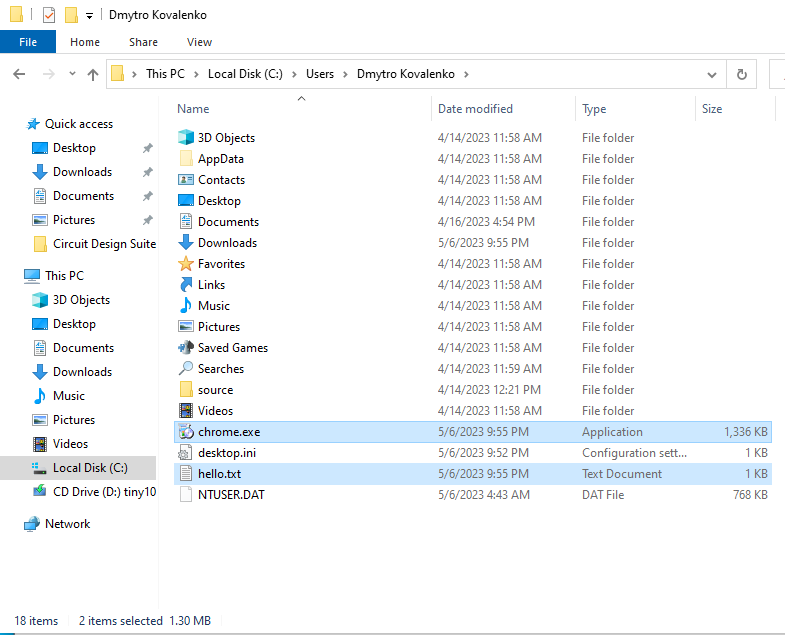
\includegraphics[width=\textwidth]{7}
	\caption{Отримані файли}
\end{figure}

\begin{figure}[H]
	\centering
	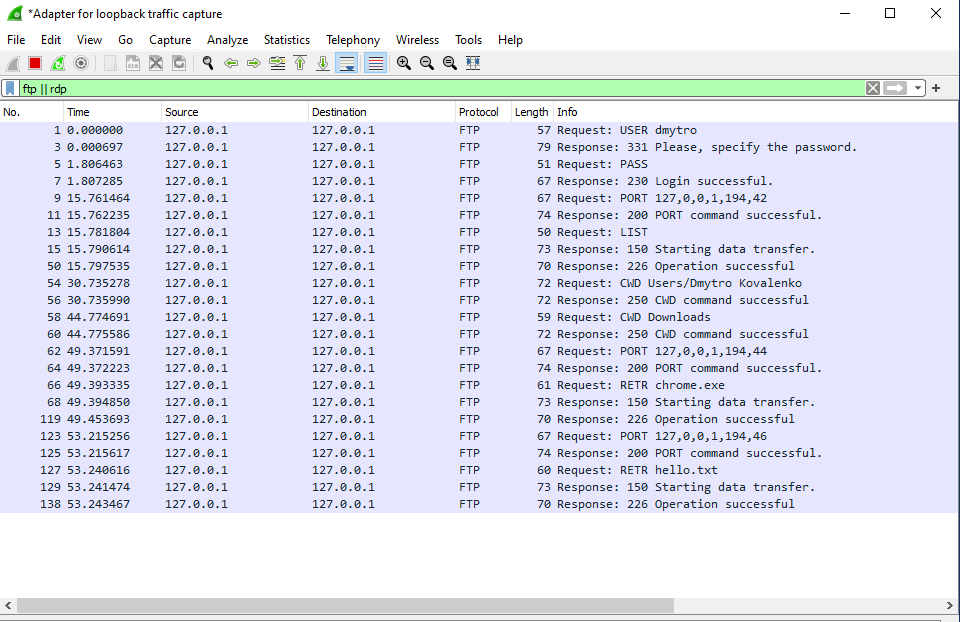
\includegraphics[width=\textwidth]{8}
	\caption{Пакети перехоплені під час взаємодії з віддаленим сервером}
\end{figure}

\section*{Висновки}
Під час виконання лабораторної роботи я ознайомився з основами протоколу FTP, дослідив формат
повідомлень FTP та принцип роботи утиліти FTP.
	    
\end{normalsize}
\end{document}
